\documentclass[a4paper, 12pt]{article}
\usepackage[a4paper,top=1.5cm, bottom=1.5cm, left=1cm, right=1cm]{geometry}
\usepackage{cmap}					
\usepackage{mathtext} 				
\usepackage[T2A]{fontenc}			
\usepackage[utf8]{inputenc}			
\usepackage[english,russian]{babel}
\usepackage{multirow}
\usepackage{graphicx}
\usepackage{wrapfig}
\usepackage{tabularx}
\usepackage{float}
\usepackage{longtable}
\usepackage{hyperref}
\hypersetup{colorlinks=true,urlcolor=blue}
\usepackage[rgb]{xcolor}
\usepackage{amsmath,amsfonts,amssymb,amsthm,mathtools} 
\usepackage{icomma} 
\usepackage{euscript}
\usepackage{mathrsfs}
\usepackage{enumerate}
\usepackage{caption}
\usepackage{enumerate}
\usepackage{graphicx}
\usepackage{caption}
\usepackage{subcaption}
\usepackage{wasysym }
\usepackage{ifthen}
\usepackage{calc}
\newcommand{\RomanNumeralCaps}[1]
    {\MakeUppercase{\romannumeral #1}}
\title{\textbf{Лабораторная раота по неорганической химии №1. Основные классы неорганических веществ и генетическая связь между ними.}}
\author{Коротков Антон и Хохлов Андрей Б06-302}
\date{10 февраля 2024}




\begin{document}

	
	\maketitle
	
	\section{Теоретическая справка}
    \begin{figure}[h]

\centering

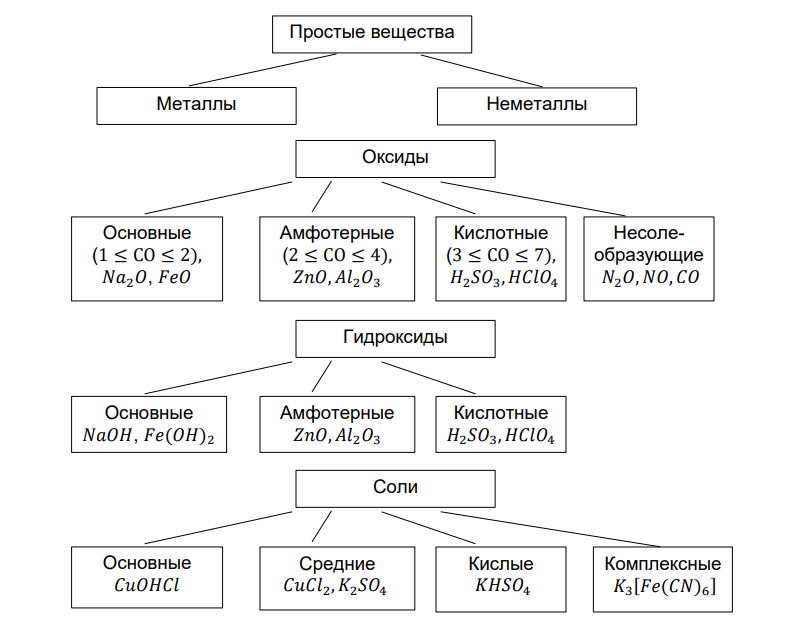
\includegraphics[width=0.8\linewidth]{2024-02-10_16-29-39.png}

\caption{Основные классы неорганических веществ}

\label{fig:mpr}

\end{figure}
\begin{figure}[H]
    \centering
    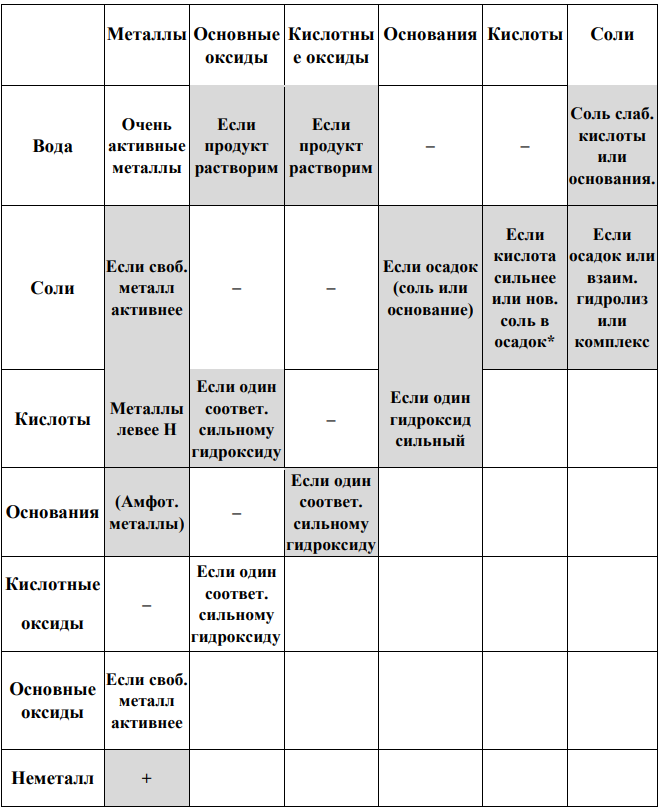
\includegraphics[width=0.8\linewidth]{2024-02-10_16-32-14.png}
    \caption{Генетическая связь между ними}
    \label{fig:enter-label}
\end{figure}

\section{Экспериментальная часть}
\subsection{Опыт №1. Взаимодействие металлов с простыми веществами.}
В нашем эксперименте цинк реагировал с серой. Сера - халькоген, в реакциях с металлами дает сульфиды или полисульфиды (полисульфиды сера может образовывать только с щелочными, щелочноземельными металлами и катионом аммония). В случае с цинком идет следующая реакция:
\begin{equation}
    Zn + S  \xrightarrow{t} ZnS + Q
\end{equation}
Реакция сопровождалась небольшим взрывом и зеленоватым пламенем. Полученное вещество было немного зеленоватое, хотя чистый сульфид цинка - белый. Такая окраска, вероятно, связана с тем, что сера прореагировала не полностью. Также после реакции чувствовался запах, похожий на запах спичек. Это диоксид серы. Судя по всему, некоторое количество сульфида цинка сгорело по следующей реакции:
\begin{equation}
    2ZnS + 3O_2 \xrightarrow{} 2ZnO + 2SO_2\uparrow + Q
\end{equation}
Стоит также отметить, что сульфид цинка(в качестве минерала) имеет несколько тривиальных названий: цинковая обманка/сфалерит и вюрцит.
\subsection{Опыт №2. Взаимодействие металлов со сложными веществами.}
Взаимодействие металлов с кислотами (в общем случае) возможно, если металл находится в ряду активности левее водорода. В ходе реакции образуется соль и выделяется водород. В своем опыте мы использовали гранулы цинка, кусочек меди и 2М соляную кислоту. Цинк, поскольку стоит в ряду активности левее водорода, будет растворяться:
\begin{equation}
    Zn + 2HCl \xrightarrow{} ZnCl_2 + H_2\uparrow
\end{equation}
При этом наблюдается растворение твердого вещества (цинка) и пузырьки выделяющегося бесцветного газа (водорода). Медь, поскольку стоит в ряду активности правее водорода, не растворяется. Вообще говоря, медь может растворятся в соляной кислоте, Но, стоит отметить, что медь может растворяться в растворах щелочных металлов при pH = 0:
]
\begin{equation}
    2Cu + 4HCl \xrightarrow{NaCl} 2H[CuCl_2] + H2\uparrow
\end{equation}
Реакция возможна за счет устойчивости данного комплекса и его малой растворимости в данных условиях. \newline
Реакция взаимодействия металлов с щелочами возможна в гораздо меньшем количестве случаев. Например, в щелочах растворяются алюминий, берилий, цинк. Растворение сопровождается образованием комплекса и выделением водорода. В нашем опыте мы растворяли гранулу алюминия в 6М едкого натра:
\begin{equation}
    2Al + 2NaOH + 6H2O \xrightarrow{} 2Na[Al(OH)_4] + 3H_2\uparrow
\end{equation}
Реакция шла довольно медленно, это связано с образованием оксидно-солевой пленки алюминием. В ходе реакции наблюдалось растворение алюминия и выделение бесцветного газа (водорода). \newline
Взаимодействие металлов с солями возможно в случае, когда более активный металл вытесняет менее активный  из его соли. В нашем случае железо вытесняет медь из ее сульфата:
\begin{equation}
    Fe + CuSO_4 \xrightarrow{} FeSO_4 + Cu\downarrow  
\end{equation}
В ходе реакции наблюдается обесцвечивание раствора (раствор сульфата меди имел характерную голубую окраску) и "покраснение" железной кнопки. Обесцвечивание связано с тем, что количество ионов меди в растворе уменьшается, а покраснение кнопки с тем, что образовавшаяся медь оседает на ней тонким слоем. Стоит также отметить, что образуется именно соль железа (\RomanNumeralCaps{2}), а не (\RomanNumeralCaps{3}). Это связано с тем, что $Cu^{2+}$ - недостаточно сильный окислитель.
\subsection{Опыт №3. Взаимодействие основных оксидов со сложными веществами.}
Основные оксиды способны реагировать с кислотами, При этом образуется соль и вода. В нашем опыте мы проводили взаимодействие оксида железа (\RomanNumeralCaps{3}) с 1М серной кислотой:
\begin{equation}
    Fe_2 O_3 + 3H_2 SO_4 \xrightarrow{} Fe_2 (SO_4 )_3 + 3H_2 O
\end{equation}
В ходе реакции наблюдается растворение твердого вещества и окрашивание раствора в сине-зеленоватый цвет. Окрашивание связано с появлением сульфата железа в растворе. \newline
Взаимодействие основных оксидов с водой (в общем случае) возможно, если образуется щелочь. Мы проводили реакцию оксида кальция с водой:
\begin{equation}
    CaO + H_2 O \xrightarrow{} Ca(OH)_2
\end{equation}
Предварительно в воду был капнут фенолфталеин, который в нейтральном растворе бесцветный. Как только мы добавили к воде оксид кальция, в растворе образовалась щелочь, среда стала щелочной, и раствор за счет фенолфталеина окрасился в малиновый цвет.
\subsection{Опыт №4. Взаимодействие кислотных оксидов со сложными веществами.}
В данном опыте мы будем пользоваться установкой, изображенной на рис.3. Она состоит из: круглодонной колбы на 250 мл, газоотводного перехода, капельной воронки, склянки Дрекселя, подсоединенной к газоотводному переходу.
\begin{figure}[h]
    \centering
    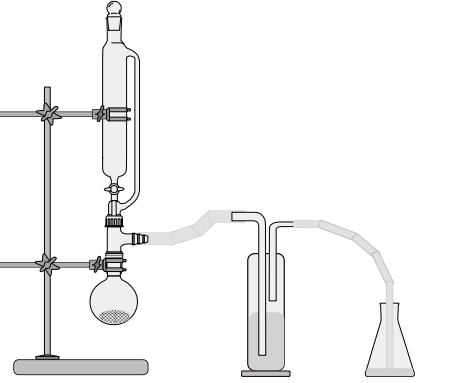
\includegraphics[width=0.55\linewidth]{2024-02-10_18-57-58.png}
    \caption{Установка}
    \label{fig:enter-label}
\end{figure}
\newline
В ходе наблюдаемого эксперимента в круглодонной колбе будет происходить растворение мраморной крошки, сопровождающееся выделением углекислого газа:
\begin{equation}
    CaCO_3 + 2HCl \xrightarrow{} CaCl_2 + CO_2\uparrow + H_2 O
\end{equation}
По газоотводной трубке углекислый газ будет переходить в склянку Дресселя, окрашивая универсальный индикатор в цвет. Далее углекислый газ идет в коническую колбу, и там наблюдается поумтенение известковой воды (качественная реакция на углекислый газ):
\begin{equation}
    Ca(OH)_2 + CO_2 \xrightarrow{} CaCO_3\downarrow + H_2 O
\end{equation}
После длительного пропускания углекислого газа происходит растворение образовавшегося осадка:
\begin{equation}
    CaCO_3 + H_2 O + CO_2 \xrightarrow{} 2Ca(HCO_3 )_2
\end{equation}
\subsection{Опыт №5. Взаимодействие кислот и оснований.}
В общем случае при взаимодействии кислот и оснований образуется соль и вода. В зависимости от избытка/недостатка могут образовываться также кислые и основные соли. В нашем опыте мы сначала добавляем в растворы едкого натра и серной кислоты универсальный индикатор. Раствор щелочи окрасится в черный цвет, а кислоты - в розовый. При добавлении к раствору гидроксида натрия серную кислоту и наоборот будет происходить следующие реакции:
\begin{equation}
    2NaOH + H_2 SO_4 \xrightarrow{} Na_2 SO_4 + 2H_2 O
\end{equation}
В пробирке с гидроксидом натрия наблюдается исчезновение окраски индикатора и затем окрашиваие раствора в розовый. В пробирке с кислотой - наоборот. 
\subsection{Опыт №6. Взаимодействие щелочей с солями и разложение оснований.}
Вобщем  случае взаимодействие солей с основаниями возможно, когда образуется слабый электролит/ комплексная соль. В нашем опыте мы рассматриваем реакцию между сульфатом меди и гидроксидом натрия, в ходе которой выпадает синий осадок:
\begin{equation}
    2NaOH + CuSO_4 \xrightarrow{} Cu(OH)_2 \downarrow + Na_2 SO_4
\end{equation}
В ходе данной реакции происходит обесцвечивание раствора сульфата меди и выпадание синего осадка гидроксида меди. Поскольку гидроксид меди - слабое основание, он является термически нестойким и при нагревании разлагается на оксид и воду:

\begin{equation}
    Cu(OH)_2 \xrightarrow{t} CuO + H_2 O
\end{equation}
В ходе данной реакции мы наблюдаемизменение цвета осадка с синего на черный, т.к. оксид меди - черное твердое вещество, не растворяющееся в воде.
\subsection{Опыт №7. Взаимодействие кислот с солями.}
В общем случае, взаимодействие кислот с солями возможно, когда более сильная кислота вытесняет более слабую из ее соли и/или в ходе этого образуется слабый электролит. В нашем опыте мы добавили к раствору хлорида бария пару капель раствора серной кислоты:
\begin{equation}
    BaCl_2 + H_2 SO_4 \xrightarrow{} BaSO_4\downarrow + HCl
\end{equation}
В ходе данной реакции образуется белый осадок сульфата бария, который не растворим ни в воде, ни в более сильных кислотых, ни в основаниях.
\subsection{Опыт №8. Гидролиз солей.}
Часть солей способна к гидролизу. ОН может быть обратимым или необратимым. В нашем опыте мы рассматриваем процессы обратимого гидролиза. Он происходит, когда соль, во-первых, растворима, а, во-вторых, ее катион/анион являются остатком слабого основания/кислоты. В нашем опыте мы исследуем среду раствора карбоната натрия. Универсальный индикатор окрашивает его раствор в черный цвет, значит, среда щелочная. Это обьясняется тем, что карбонат-ион - остаток слабой угольной кислоты, а катион натрия - остаток сильного основания. Поэтому гидролиз идет по аниону и среда щеллочная:
\begin{equation}
    Na_2 CO_3 + H_2 O \xleftrightarrow{}{} NaHCO_3 +NaOH 
\end{equation}
\begin{equation}
    NaHCO_3 + H_2 O \xleftrightarrow{}{}  H_2 CO_3 + NaOH 
\end{equation}
\begin{equation}
    CO_3^{2-} + 2H_2 O \xleftrightarrow{}{} H_2 CO_3 + 2 OH^{-}
\end{equation}
У сульфата меди наоборот, гидролиз по аниону и среда кислая. Индикатор окрашивается в розовый цвет:
\begin{equation}
    2CuSO_4 + 2H2O \xleftrightarrow{}{} (CuOH)_2 SO_4 + H_2 SO_4
\end{equation}
\begin{equation}
    (CuOH)_2 SO_4 + 2H_2 O \xleftrightarrow{}{}  2Cu(OH)_2 + H_2 SO_4
\end{equation}
\begin{equation}
    Cu^{2+} + 2H_2 O \xleftrightarrow{}{}  Cu(OH)_2 + 2H^{+}
\end{equation}
\subsection{Опыт №9. Взаимодействие солей друг с другом.}
Соли в общем случае реагируют дург с другом, когда в ходе реакции образуется слабый электролит или комплексное соединение. В нашем опыте в первом случае мы рассмотрим реакцию между карбонатом натрия и хлоридом кальция, в ходе которой образуется белый осадока карбоната кальция, и реакцию хлорида натрия и сульфата меди, в ходе которой образуется комплекс меди, окрашивающий раствор в зеленый цвет:
\begin{equation}
    CaCl_2 + Na_2 CO_3 \xrightarrow{} CaCO_3 + 2NaCl
\end{equation}
\begin{equation}
    CuSO_4 + 4NaCL \xrightarrow{} Na_2 [CuCl_4] + Na_2 SO_4
\end{equation}
\section{Вывод}
Мы повторили основные классы неорганических веществ, провели реакции между ними, на практике увидели цвета некоторых осадков и растворов.
    

\end{document}

